\documentclass[12pt,a4paper]{article}
\usepackage[utf8]{inputenc}
\usepackage[english]{babel}
\usepackage[margin=1in]{geometry}
\usepackage{graphicx}
\usepackage{tikz}
\usepackage{listings}
\usepackage{booktabs}
\usepackage{float}
\usepackage{enumitem}

% Simple TikZ setup
\usetikzlibrary{shapes,arrows,positioning}

% Basic code listing style
\lstset{
    basicstyle=\footnotesize\ttfamily,
    frame=single,
    breaklines=true,
    numbers=left,
    numberstyle=\tiny
}

\title{\textbf{Air Cargo Booking \& Tracking System}\\
       \large System Design Document}
\author{Kesha\\
        Computer Science Student}
\date{\today}

\begin{document}

\maketitle

\tableofcontents
\newpage

\section{Introduction}

This document describes the design of an Air Cargo Booking and Tracking System developed as a web application. The system allows users to book cargo shipments and track them in real-time.

\subsection{Project Overview}
The Air Cargo System is a full-stack web application that provides:
\begin{itemize}
    \item User registration and authentication
    \item Flight route searching
    \item Cargo booking management
    \item Real-time shipment tracking
\end{itemize}

\subsection{Technologies Used}
\begin{itemize}
    \item \textbf{Frontend:} React with TypeScript, Material-UI
    \item \textbf{Backend:} Node.js with Express
    \item \textbf{Database:} PostgreSQL
    \item \textbf{Authentication:} JWT (JSON Web Tokens)
    \item \textbf{Database ORM:} Sequelize/TypeORM
\end{itemize}

\section{System Architecture}

\subsection{Overall Architecture}
The system follows a typical 3-tier architecture:

\begin{figure}[H]
\centering
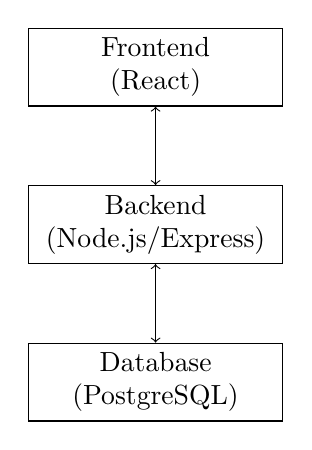
\begin{tikzpicture}[node distance=2cm]
    \node (frontend) [rectangle, draw, text width=3cm, text centered] {Frontend\\(React)};
    \node (backend) [rectangle, draw, text width=3cm, text centered, below of=frontend] {Backend\\(Node.js/Express)};
    \node (database) [rectangle, draw, text width=3cm, text centered, below of=backend] {Database\\(PostgreSQL)};
    
    \draw [<->] (frontend) -- (backend);
    \draw [<->] (backend) -- (database);
\end{tikzpicture}
\caption{System Architecture}
\end{figure}

\subsection{Component Structure}

\subsubsection{Frontend Components}
\begin{itemize}
    \item Authentication (Login/Signup)
    \item Dashboard
    \item Route Search
    \item Booking Management
    \item Tracking Interface
\end{itemize}

\subsubsection{Backend Components}
\begin{itemize}
    \item Authentication Controller
    \item Route Controller
    \item Booking Controller
    \item Database Models
    \item Middleware (Auth, Error Handling)
\end{itemize}

\section{Database Design}

\subsection{Database Tables}

The system uses 5 main tables:

\begin{table}[H]
\centering
\begin{tabular}{@{}ll@{}}
\toprule
\textbf{Table} & \textbf{Purpose} \\
\midrule
users & Store user account information \\
airlines & Store airline data \\
flights & Store flight information \\
bookings & Store booking records \\
timeline\_events & Store tracking events \\
\bottomrule
\end{tabular}
\caption{Database Tables}
\end{table}

\subsection{Key Relationships}
\begin{itemize}
    \item Users can have multiple bookings
    \item Bookings are linked to specific flights
    \item Timeline events track booking status changes
\end{itemize}

\section{API Design}

\subsection{Main API Endpoints}

\begin{table}[H]
\centering
\small
\begin{tabular}{@{}lll@{}}
\toprule
\textbf{Method} & \textbf{Endpoint} & \textbf{Description} \\
\midrule
POST & /api/v1/auth/signup & User registration \\
POST & /api/v1/auth/login & User login \\
GET & /api/v1/routes & Search flight routes \\
POST & /api/v1/bookings & Create booking \\
GET & /api/v1/bookings/my-bookings & Get user bookings \\
GET & /api/v1/bookings/:id/history & Get booking history \\
\bottomrule
\end{tabular}
\caption{Main API Endpoints}
\end{table}

\subsection{API Response Format}
All API responses use a standard JSON format:

\begin{lstlisting}[caption=API Response Example]
{
  "message": "Operation successful",
  "data": {
    // Response data here
  }
}
\end{lstlisting}

\section{Key Features}

\subsection{User Authentication}
\begin{itemize}
    \item Users can register with email and password
    \item Secure login using JWT tokens
    \item Password hashing with bcrypt
\end{itemize}

\subsection{Route Search}
\begin{itemize}
    \item Search available flights between cities
    \item Display flight details (airline, times, etc.)
    \item Support for multi-leg journeys
\end{itemize}

\subsection{Booking Management}
\begin{itemize}
    \item Create new cargo bookings
    \item Specify cargo details (weight, pieces)
    \item Select flight routes
    \item Generate unique booking reference
\end{itemize}

\subsection{Tracking System}
\begin{itemize}
    \item Real-time status updates
    \item Timeline view of events
    \item Status types: Created, Departed, Arrived, Delivered
\end{itemize}

\section{Implementation Details}

\subsection{Security Features}
\begin{itemize}
    \item JWT-based authentication
    \item Password encryption
    \item Input validation on all forms
    \item Protected API routes
\end{itemize}

\subsection{User Interface}
\begin{itemize}
    \item Responsive design using Material-UI
    \item Clean and simple navigation
    \item Form validation with error messages
    \item Loading states for better UX
\end{itemize}

\subsection{Development Setup}
Basic commands to run the project:

\begin{lstlisting}[caption=Development Commands]
# Backend
cd backend
npm install
npm run dev

# Frontend  
cd frontend
npm install
npm start
\end{lstlisting}

\section{Testing}

\subsection{Testing Approach}
\begin{itemize}
    \item Manual testing of all features
    \item API testing using Postman
    \item Browser testing for UI components
    \item Database functionality verification
\end{itemize}

\subsection{Test Cases}
\begin{enumerate}
    \item User registration and login
    \item Route search functionality
    \item Booking creation process
    \item Tracking status updates
    \item Error handling scenarios
\end{enumerate}

\section{Challenges \& Solutions}

\subsection{Technical Challenges}
\begin{itemize}
    \item \textbf{State Management:} Used Redux for complex state handling
    \item \textbf{Authentication:} Implemented JWT for secure sessions
    \item \textbf{Database Design:} Created normalized schema for efficiency
    \item \textbf{Error Handling:} Added comprehensive error management
\end{itemize}

\subsection{Learning Outcomes}
\begin{itemize}
    \item Gained experience with full-stack development
    \item Learned modern React patterns and hooks
    \item Understanding of RESTful API design
    \item Database modeling and relationship design
\end{itemize}

\section{Future Improvements}

\subsection{Possible Enhancements}
\begin{itemize}
    \item Email notifications for status updates
    \item Mobile app version
    \item Advanced reporting features
    \item Integration with real airline APIs
    \item Payment processing system
\end{itemize}

\subsection{Scalability Considerations}
\begin{itemize}
    \item Migration from SQLite to PostgreSQL
    \item Implementation of caching
    \item Load balancing for high traffic
    \item Microservices architecture
\end{itemize}

\subsection{Database Choice - PostgreSQL}
\begin{itemize}
    \item \textbf{Production-Ready:} Industry standard database
    \item \textbf{ACID Compliance:} Reliable transactions
    \item \textbf{Advanced Features:} JSON support, full-text search
    \item \textbf{Scalability:} Better performance for large datasets
    \item \textbf{Cloud Options:} Can use free hosted services (ElephantSQL, Heroku)
\end{itemize}

\section{Conclusion}

The Air Cargo Booking and Tracking System successfully demonstrates a complete web application with modern technologies. The project covers all essential aspects of full-stack development including:

\begin{itemize}
    \item Frontend development with React and TypeScript
    \item Backend API development with Node.js
    \item Database design and management
    \item User authentication and security
    \item Real-time data tracking
\end{itemize}

This project has provided valuable hands-on experience with industry-standard tools and practices, preparing for real-world software development challenges.

The system is functional and ready for demonstration, showcasing both technical skills and understanding of software architecture principles.

\vspace{1cm}
\hrule
\begin{center}
\textit{End of Document}\\
Air Cargo System Design\\
Student Project - \today
\end{center}

\end{document}